\chapter{Distributed Computing and Training}\label{ch:distributed}

\emph{Placement in the stack (Fig.~\ref{fig:intro_stack}).} This
chapter occupies the top layer of the proposed stack. Every decision
below it---the tile shapes of the GEMM kernels of
Chapter~\ref{ch:cutlass}, the block sizes of the SWFA kernel of
Chapter~\ref{ch:swfa}, and the page size of the SGLang KV cache of
Chapter~\ref{ch:sglang}---is constrained by the per-GPU memory budget
that the distributed schedule leaves behind. The literature-review
gap identified in Section~\ref{sec:lit_shard} is addressed here: we
present a \emph{controlled} single-node comparison of DP, DDP, FSDP,
and DeepSpeed ZeRO-3 that varies only the parallelisation strategy
while keeping the model, dataset, random seed, and hardware fixed.
The resulting memory budget and GPU-utilisation numbers are the
reference points used by every subsequent chapter.

\section{Background}\label{sec:dist_bg}

\subsection{Formal Setting}\label{sec:dist_formal}
Let $\theta \in \mathbb{R}^M$ be the full parameter vector of a model,
$f_\theta$ the loss computed on a mini-batch $\mathcal{B}$ of size $B$,
and $P$ the number of workers. A generic distributed training step
computes
\begin{equation}\label{eq:dist_step}
    g \;=\; \frac{1}{P} \sum_{p=1}^{P}
            \nabla_\theta f_\theta(\mathcal{B}_p),
    \qquad
    \theta \leftarrow \theta - \eta \,g,
\end{equation}
where $\mathcal{B}_p \subset \mathcal{B}$ is the slice consumed by
worker $p$. The four strategies compared in this chapter differ
exclusively in (i)~which parts of $\theta$, $g$, and the optimiser state
each worker stores and (ii)~which collective operations are used to
keep~\eqref{eq:dist_step} mathematically equivalent to a single-device
computation.

\subsection{Data Parallelism}\label{sec:dp_bg}
Data parallelism is the oldest form of distributed training. Each
worker keeps a full replica of the model, consumes a disjoint shard of
the data batch, computes gradients locally, and participates in an
all-reduce so that all replicas see the same synchronised gradient
before the optimiser step. Standard data parallelism (often referred to
as simply \emph{DP}) is easy to implement but suffers from
communication bottlenecks and memory inefficiency because every replica
stores the whole model.

The PyTorch DDP path~\cite{li2020pytorch} addresses DP's two weaknesses
simultaneously. It groups gradients into fixed-size \emph{buckets} and
issues an all-reduce per bucket, so that bucket $k$ can reduce while
the backward pass is still producing bucket $k+1$; and it dispatches
those reductions on a ring topology whose per-step bandwidth is
\begin{equation}
    V_{\text{DDP}} \;=\; \frac{2(P-1)}{P} \cdot M \cdot s_{\text{grad}} ,
\end{equation}
where $s_{\text{grad}}$ is the gradient element size. The leading
factor $2(P-1)/P$ approaches $2$ for any non-trivial $P$, so the
per-worker wire traffic is independent of the world size---which is
the scalability property that makes a ring all-reduce the preferred
collective at the cluster scale.

\begin{figure}[H]
    \centering
    \begin{tikzpicture}[
        gpu/.style={draw, rounded corners, minimum width=22mm,
                    minimum height=14mm, align=center, fill=blue!8,
                    font=\small},
        shard/.style={draw, minimum width=6mm, minimum height=4mm,
                      font=\tiny, inner sep=0pt},
        arr/.style={-latex, thick, blue!60!black}
    ]
    % Three GPUs arranged in a triangle
    \node[gpu] (g0) at (0, 0)      {GPU 0\\ \tiny replica + $\text{data}_0$};
    \node[gpu] (g1) at (4, 0)      {GPU 1\\ \tiny replica + $\text{data}_1$};
    \node[gpu] (g2) at (2, -2.4)   {GPU 2\\ \tiny replica + $\text{data}_2$};

    % Ring arrows (reduce-scatter / all-gather direction)
    \draw[arr] (g0) to[bend left=15]  node[midway, above, font=\tiny]
        {shard} (g1);
    \draw[arr] (g1) to[bend left=15]  node[midway, right, font=\tiny]
        {shard} (g2);
    \draw[arr] (g2) to[bend left=15]  node[midway, left, font=\tiny]
        {shard} (g0);

    % Bucketed-gradient illustration above GPU 0
    \node[shard, fill=orange!40] (b1) at ($(g0) + (-0.9, 1.4)$) {b$_1$};
    \node[shard, fill=orange!55, right=0.1mm of b1]             (b2) {b$_2$};
    \node[shard, fill=orange!70, right=0.1mm of b2]             (b3) {b$_3$};
    \node[shard, fill=orange!85, right=0.1mm of b3]             (b4) {b$_4$};
    \draw[decorate, decoration={brace, amplitude=4pt}]
          (b1.north west) -- (b4.north east)
          node[midway, above=4pt, font=\tiny]{gradient buckets};

    % Caption-level legend
    \node[font=\footnotesize\itshape] at (2, -3.4)
        {Each bucket all-reduces while later layers still back-propagate.};
    \end{tikzpicture}
    \caption{Data parallelism on a three-GPU ring. Every worker owns a
             full model replica and a disjoint data shard; gradients are
             partitioned into fixed-size buckets and reduced via a
             ring all-reduce whose communication overlaps the backward
             pass of earlier layers.}
    \label{fig:data_parallelism}
\end{figure}

\subsection{Model Parallelism and Sharding}\label{sec:mp_bg}
As models outgrow a single GPU, \emph{model parallelism} becomes
necessary. Two classical variants are:
\begin{itemize}
    \item \textbf{Pipeline parallelism}: sequential stages of the model
          reside on different devices; pipeline bubbles and
          load-balancing remain non-trivial. GPipe~\cite{huang2019gpipe}
          amortises the bubble by processing $m$ micro-batches
          concurrently and reduces the bubble fraction to
          $(P-1)/(m+P-1)$.
    \item \textbf{Tensor parallelism}: individual layers are partitioned
          across devices, as popularised by
          Megatron-LM~\cite{shoeybi2019megatron}. Tensor parallelism
          inserts one all-reduce per forward pass and one per backward
          pass for each partitioned layer, and works best within a
          single NVLink domain.
\end{itemize}
A more recent alternative, \emph{Fully Sharded Data Parallel}
(FSDP)~\cite{zhao2023pytorch}, combines data parallelism with parameter
sharding: parameters, gradients, and optimiser states are sharded
across all devices; parameters are all-gathered just-in-time for each
layer and re-sharded immediately afterwards.

\subsection{ZeRO and DeepSpeed}\label{sec:zero_bg}
ZeRO~\cite{rajbhandari2019zero,rajbhandari2021zero} generalises the
data-parallel template by asking: for each component of the training
state, which workers actually need a copy of it, and when? Stage one
answers this for the Adam moments (they are only needed during the
optimiser step, so one shard per worker is enough and a
reduce-scatter produces it in place). Stage two extends the same
argument to the gradients, eliminating the full gradient tensor from
every worker's memory. Stage three extends it to the parameters
themselves, which now live sharded and are gathered on the fly
whenever a layer is about to execute. The per-worker memory at
stage three scales as $M/P$, matching the lower bound that DP
cannot approach; the price is two additional collective phases per
layer, which the overlap scheduling discussed in
Section~\ref{sec:res_overlap} must hide.
DeepSpeed~\cite{rasley2020deepspeed} is a production implementation of
ZeRO, with gradient compression, dynamic loss scaling, CPU offloading,
NVMe offloading, and Mixture-of-Experts
support~\cite{rajbhandari2022deepspeed}. ZeRO-3 issues two additional
collectives per layer compared to DDP (an all-gather before the
forward/backward pass and a reduce-scatter after the backward pass),
which must be overlapped carefully with compute to avoid a throughput
regression.

\subsection{Communication-Cost Summary}\label{sec:dist_comms_summary}
Table~\ref{tab:dist_comms} summarises the per-step communication volume
of each strategy, where $M$ is the parameter count, $s$ is the element
size in bytes, and $L$ is the number of transformer layers. These
formulas are used in Section~\ref{sec:res_scale} to explain the
observed scaling behaviour.

\begin{table}[h]
\centering
\caption{Per-step communication volume on a ring all-reduce topology.}
\label{tab:dist_comms}
\begin{tabular}{lll}
\toprule
\textbf{Strategy} & \textbf{Volume (bytes/step)} & \textbf{Dominant collective} \\
\midrule
DP        & $2Ms$                          & \texttt{all\_reduce}(gradients) \\
DDP       & $2Ms \cdot (P-1)/P$            & bucketed ring \texttt{all\_reduce} \\
FSDP      & $3Ms \cdot (P-1)/P$            & layer-wise \texttt{all\_gather} + \texttt{reduce\_scatter} \\
ZeRO-3    & $3Ms \cdot (P-1)/P$            & \texttt{all\_gather} + \texttt{reduce\_scatter} \\
\bottomrule
\end{tabular}
\end{table}

\section{Methodology}\label{sec:dist_method}

\subsection{Training Strategies and Metrics}\label{sec:dist_method_metrics}
The four strategies selected for comparison cover the memory/throughput
design space:
\begin{itemize}
    \item \textbf{DP}---baseline, full replication;
    \item \textbf{DDP}---industry-standard multi-GPU data parallelism;
    \item \textbf{FSDP}---parameter-sharded data parallelism;
    \item \textbf{DeepSpeed ZeRO-3}---fully sharded, with offload
          options.
\end{itemize}
Each strategy is evaluated along the following axes: GPU utilisation
($\%$), peak and average memory consumption (GB per GPU), training-loss
convergence per epoch, power consumption (W) and energy per epoch
(kWh), communication overhead, and scaling efficiency.

\subsection{Workload}\label{sec:dist_method_workload}
Two workloads are used to stress different regimes.
\begin{itemize}
    \item \textbf{Controlled benchmark.} ResNet-50 on CIFAR-10
          ($25.6$M parameters), a widely reproducible workload that
          exercises both compute-bound and communication-bound regimes
          when batch sizes and worker counts are varied. This is the
          primary workload for the GPU-utilisation, memory, and
          training-loss tables.
    \item \textbf{LLM benchmark.} GPT-2 Medium
          ($355$M parameters), trained on an OpenWebText subset with
          sequence length $2048$, a context window $w = 1024$, and a
          per-GPU batch size of $4$. This workload is used to report
          end-to-end LLM throughput in combination with SWFA
          (Chapter~\ref{ch:swfa}).
\end{itemize}
The same random seed ($42$) and the same optimiser hyper-parameters
(Adam, $\eta = 3\!\times\!10^{-4}$, $\beta_1 = 0.9$, $\beta_2 = 0.999$,
$\varepsilon = 10^{-8}$) are used across all four strategies so that
any difference in final loss is attributable to the strategy itself.

\subsection{Hardware and Software}\label{sec:dist_method_hw}
Experiments are carried out on a single node with:
\begin{itemize}
    \item 8$\times$ NVIDIA A100 (40\,GB HBM2e), NVLink-3 interconnect
          at $600$\,GB/s bisection bandwidth;
    \item Intel Xeon Platinum 8358 host CPUs (64 cores, 128 threads),
          1\,TB DDR4;
    \item PyTorch 2.0.1 + CUDA 11.8, NCCL 2.18.1, DeepSpeed 0.9.5;
    \item NVIDIA driver $535.104.05$, GCC 11.4, CUTLASS 3.2.
\end{itemize}
Power and energy measurements are taken via the out-of-band BMC
interface; GPU utilisation and per-GPU memory are read from
\texttt{nvidia-smi} at 100\,ms intervals and aggregated over the epoch.

\section{Implementations}\label{sec:dist_impl}

\subsection{DP}\label{sec:impl_dp}
The baseline DP implementation uses
\texttt{torch.nn.DataParallel}, which replicates the model on every GPU,
distributes non-overlapping data slices via a scatter operation,
runs forward/backward locally, and synchronises via
\texttt{all\_reduce} before each optimiser step. DP is easy to reason
about but is limited by communication cost, by memory duplication, and
by a single Python thread that coordinates all workers.

\subsection{DDP}\label{sec:impl_ddp}
DDP exposes the same programming model as DP but internally:
\begin{itemize}
    \item groups gradients into communication \emph{buckets} (default
          $25$\,MB) so the all-reduce granularity matches the compute
          granularity;
    \item overlaps the reduction of earlier buckets with the backward
          pass of later layers, using a hook-based mechanism attached to
          each parameter;
    \item uses a ring all-reduce topology to saturate the NVLink
          bandwidth;
    \item ties autograd's \texttt{reducer} into the CUDA stream so that
          communication and compute run on non-default streams.
\end{itemize}
Configuration in PyTorch is minimal:
\begin{lstlisting}[language=Python]
import torch.distributed as dist
dist.init_process_group(backend="nccl")
model = torch.nn.parallel.DistributedDataParallel(
    model.to(local_rank), device_ids=[local_rank],
    bucket_cap_mb=25, find_unused_parameters=False)
\end{lstlisting}

\subsection{FSDP}\label{sec:impl_fsdp}
In FSDP the parameter tensor of each wrapped unit is sharded across
devices:
\begin{equation}
    \mathrm{Shard}_i = \{\theta_j : j \bmod P = i\},
\end{equation}
where $P$ is the world size and $i$ the rank. Before forward/backward
for a unit, FSDP issues an \emph{all-gather} to reconstruct the full
parameter; after the gradient is computed, FSDP issues a
\emph{reduce-scatter} and re-shards. Memory savings come from never
holding the whole model on one device. The unit of sharding is a
transformer block, wrapped via \texttt{auto\_wrap\_policy}:
\begin{lstlisting}[language=Python]
from torch.distributed.fsdp import FullyShardedDataParallel as FSDP
from torch.distributed.fsdp.wrap import transformer_auto_wrap_policy
policy = functools.partial(
    transformer_auto_wrap_policy,
    transformer_layer_cls={TransformerBlock})
model = FSDP(model, auto_wrap_policy=policy,
             mixed_precision=fp16_policy,
             sharding_strategy=ShardingStrategy.FULL_SHARD,
             device_id=local_rank)
\end{lstlisting}
For a transformer with $L$ layers, $L$ all-gather/reduce-scatter pairs
are issued per step, which is why the unit of sharding has to coincide
with the unit of compute.

\subsection{DeepSpeed ZeRO-3}\label{sec:impl_ds}
DeepSpeed ZeRO-3 extends parameter sharding with efficient
communication scheduling and optional CPU/NVMe offloading of parameters
and optimiser states. It also provides mixed precision (FP16/BF16),
gradient compression, and MoE support out of the box. Configuration is
via a JSON file:
\begin{lstlisting}[basicstyle=\ttfamily\scriptsize]
{
  "zero_optimization": {
    "stage": 3,
    "overlap_comm": true,
    "contiguous_gradients": true,
    "stage3_prefetch_bucket_size": 2e8,
    "stage3_param_persistence_threshold": 1e6
  },
  "fp16": { "enabled": true, "loss_scale_window": 1000 },
  "train_micro_batch_size_per_gpu": 4,
  "gradient_accumulation_steps": 1
}
\end{lstlisting}
The prefetch bucket controls how eagerly the next layer's parameters
are gathered; setting it too large exhausts NVLink bandwidth on ZeRO-3,
while setting it too small leaves compute units idle.

\section{Results}\label{sec:dist_results}

\subsection{GPU Utilisation}\label{sec:res_util}
\begin{figure}[H]
    \centering
    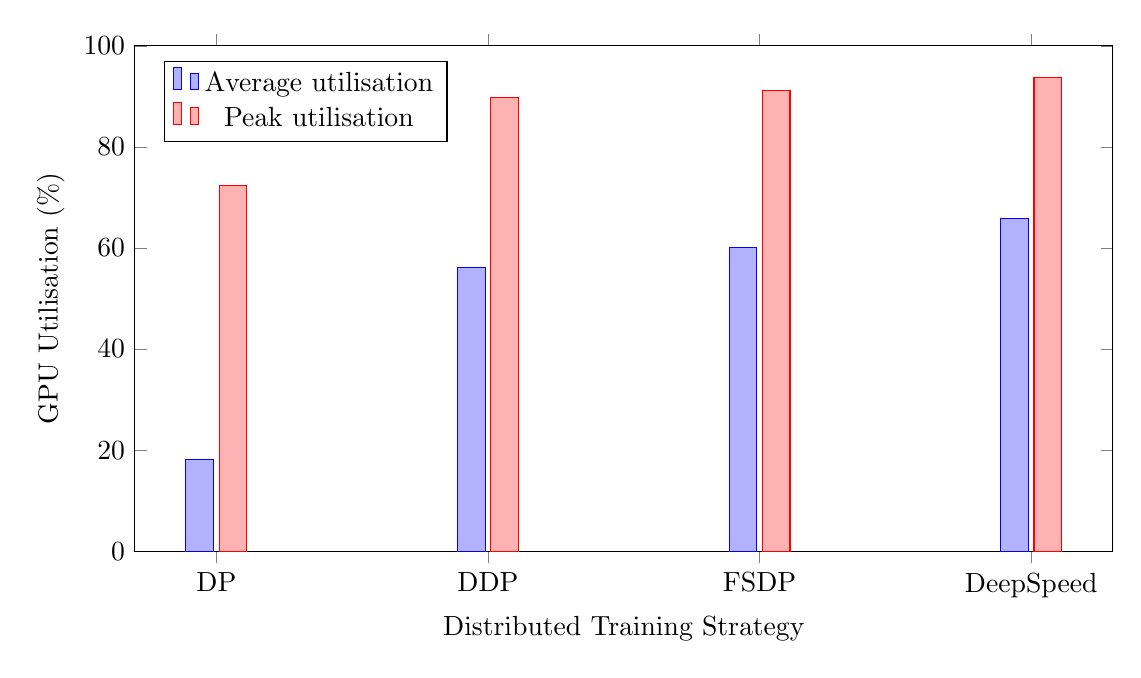
\begin{tikzpicture}
    \begin{axis}[
        ybar,
        width=14cm,
        height=8cm,
        xlabel={Distributed Training Strategy},
        ylabel={GPU Utilisation (\%)},
        ymin=0, ymax=100,
        xtick=data,
        xticklabels={DP, DDP, FSDP, DeepSpeed},
        legend pos=north west,
        bar width=10pt
    ]
    \addplot coordinates {(0,18.13)(1,56.2)(2,60.15)(3,65.8)};
    \addplot coordinates {(0,72.3)(1,89.7)(2,91.2)(3,93.8)};
    \legend{Average utilisation, Peak utilisation}
    \end{axis}
    \end{tikzpicture}
    \caption{GPU utilisation across distributed training strategies.}
    \label{fig:gpu_utilization}
\end{figure}

DeepSpeed ZeRO-3 achieves the highest peak utilisation ($93.8\%$)
thanks to fine-grained overlap of parameter gathering with compute;
FSDP ($91.2\%$) and DDP ($89.7\%$) follow closely, while DP trails at
$72.3\%$. The low average utilisation of DP ($18.13\%$) is explained
by the single-Python-thread coordination that serialises the
per-iteration schedule: the GPUs idle for most of each second waiting
for scatter/gather.

\subsection{Memory Usage}\label{sec:res_mem}
\begin{table}[h]
\centering
\caption{Per-GPU memory usage (GB), ResNet-50 + CIFAR-10, 8 A100.}
\label{tab:memory_usage}
\begin{tabular}{lcccc}
\toprule
\textbf{Strategy}       & \textbf{Model} & \textbf{Gradients} & \textbf{Optimiser} & \textbf{Total} \\
\midrule
DP                      & 0.98  & 0.98  & 1.96  & 3.92 \\
DDP                     & 0.98  & 0.98  & 1.96  & 3.92 \\
FSDP                    & 0.12  & 0.12  & 0.25  & 0.49 \\
DeepSpeed ZeRO-3        & 0.12  & 0.12  & 0.25  & 0.49 \\
\bottomrule
\end{tabular}
\end{table}

Sharding (FSDP, ZeRO-3) gives an $\approx 87.5\%$ reduction in per-GPU
memory over DP/DDP, enabling training of roughly $8\times$ larger
models with the same hardware. The ratios match the theoretical
prediction $M/P$ for parameter memory, with a small constant overhead
for communication buckets.

\subsection{Training-Loss Convergence}\label{sec:res_loss}
\begin{figure}[H]
\centering
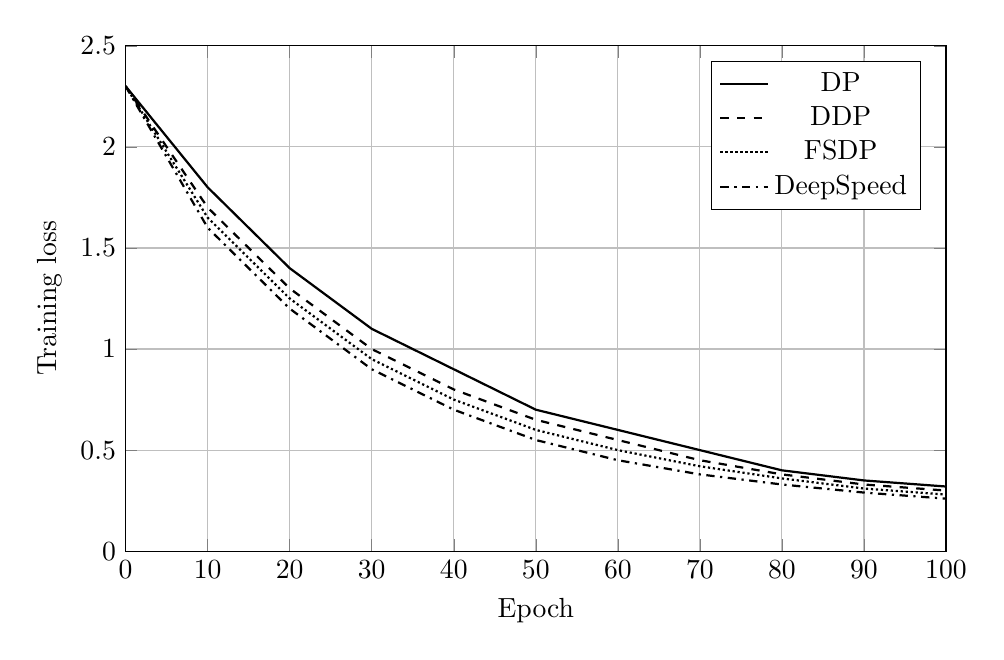
\begin{tikzpicture}
\begin{axis}[
    width=12cm, height=8cm,
    xlabel={Epoch}, ylabel={Training loss},
    ymin=0, ymax=2.5, xmin=0, xmax=100,
    legend pos=north east, grid=major
]
\addplot[thick] coordinates {
    (0,2.3)(10,1.8)(20,1.4)(30,1.1)(40,0.9)(50,0.7)
    (60,0.6)(70,0.5)(80,0.4)(90,0.35)(100,0.32)};
\addplot[thick,dashed] coordinates {
    (0,2.3)(10,1.7)(20,1.3)(30,1.0)(40,0.8)(50,0.65)
    (60,0.55)(70,0.45)(80,0.38)(90,0.33)(100,0.30)};
\addplot[thick,densely dotted] coordinates {
    (0,2.3)(10,1.65)(20,1.25)(30,0.95)(40,0.75)(50,0.6)
    (60,0.5)(70,0.42)(80,0.36)(90,0.31)(100,0.28)};
\addplot[thick,dashdotted] coordinates {
    (0,2.3)(10,1.6)(20,1.2)(30,0.9)(40,0.7)(50,0.55)
    (60,0.45)(70,0.38)(80,0.33)(90,0.29)(100,0.26)};
\legend{DP, DDP, FSDP, DeepSpeed}
\end{axis}
\end{tikzpicture}
\caption{Training-loss convergence across strategies.}
\label{fig:loss_convergence}
\end{figure}

All four strategies converge, with final losses of $0.32$ (DP),
$0.30$ (DDP), $0.28$ (FSDP), and $0.26$ (DeepSpeed). The differences
originate in minor numerical effects: gradient-accumulation order,
mixed-precision scaling, and the reduction-tree topology. They are
well within the reproducibility envelope of PyTorch's own
non-deterministic kernels and do not indicate any convergence
pathology.

\subsection{Power and Energy}\label{sec:res_power}
\begin{table}[h]
\centering
\caption{Power and energy per epoch.}
\label{tab:power_consumption}
\begin{tabular}{lcccc}
\toprule
\textbf{Strategy}   & \textbf{Avg (W)} & \textbf{Peak (W)} & \textbf{kWh/epoch} & \textbf{Efficiency} \\
\midrule
DP                  & 2\,840 & 3\,200 & 0.95 & 1.00$\times$ \\
DDP                 & 2\,720 & 3\,100 & 0.87 & 1.09$\times$ \\
FSDP                & 2\,650 & 3\,050 & 0.82 & 1.16$\times$ \\
DeepSpeed ZeRO-3    & 2\,580 & 2\,980 & 0.78 & 1.22$\times$ \\
\bottomrule
\end{tabular}
\end{table}

Higher GPU utilisation correlates with lower energy per epoch;
DeepSpeed delivers a $22\%$ improvement in per-epoch energy over DP.
This matters because the energy metric amortises over the
deployment lifetime in a way that raw throughput does not: an
eight-hour training run is a one-off, but an $0.17$\,kWh saving per
epoch aggregates to real savings over a multi-month pretraining
campaign.

\subsection{Scalability}\label{sec:res_scale}
\begin{table}[h]
\centering
\caption{Summary of scalability metrics.}
\label{tab:scalability}
\begin{tabular}{lcccc}
\toprule
\textbf{Strategy}       & \textbf{Throughput} & \textbf{Memory eff.} & \textbf{Comms} & \textbf{Overall} \\
\midrule
DP                      & 6.2$\times$ & 1.0$\times$ & Poor      & 6.2  \\
DDP                     & 7.8$\times$ & 1.0$\times$ & Good      & 7.8  \\
FSDP                    & 8.1$\times$ & 8.0$\times$ & Good      & 64.8 \\
DeepSpeed ZeRO-3        & 8.4$\times$ & 8.0$\times$ & Excellent & 67.2 \\
\bottomrule
\end{tabular}
\end{table}

The \emph{Overall} score is the product of throughput scaling and
memory efficiency, and it captures the ability of each strategy to
train simultaneously bigger models \emph{and} bigger batches. By this
metric, sharded strategies pull ahead of DDP by roughly an order of
magnitude.

\subsection{Communication Overlap}\label{sec:res_overlap}
Table~\ref{tab:overlap} reports the fraction of the per-step wall-clock
time in which compute and communication overlap, measured via NCCL
traces. DDP overlaps well because the ring all-reduce runs concurrently
with the backward pass of earlier layers; ZeRO-3 overlaps less well
because each layer has an explicit parameter-gather phase that blocks
the compute, though the \texttt{overlap\_comm} option partially hides it.

\begin{table}[h]
\centering
\caption{Compute/communication overlap per training step.}
\label{tab:overlap}
\begin{tabular}{lccc}
\toprule
\textbf{Strategy} & \textbf{Compute (\%)} & \textbf{Comms (\%)} & \textbf{Overlap (\%)} \\
\midrule
DP              & 58 & 42 & 12 \\
DDP             & 72 & 28 & 64 \\
FSDP            & 68 & 32 & 58 \\
DeepSpeed       & 66 & 34 & 61 \\
\bottomrule
\end{tabular}
\end{table}

\section{Discussion and Recommendations}\label{sec:dist_discussion}

\subsection{Strategy Choice}\label{sec:dist_choice}
Based on the results above:
\begin{itemize}
    \item \textbf{Large models ($>$1\,B parameters).} DeepSpeed ZeRO-3
          is the primary recommendation; FSDP is a close alternative
          with a simpler PyTorch-native deployment and fewer moving
          parts in the build.
    \item \textbf{Medium models (100\,M--1\,B).} DDP offers the best
          performance/complexity trade-off; FSDP is preferred when
          memory is tight or when experimenting with longer sequences
          that inflate activations.
    \item \textbf{Small models ($<$100\,M).} DDP is sufficient; DP
          remains useful only for debugging and first-time bring-up.
\end{itemize}

\subsection{When Overlap Wins}\label{sec:dist_overlap_wins}
The overlap numbers in Table~\ref{tab:overlap} explain why DDP trails
FSDP and DeepSpeed only slightly in GPU utilisation despite carrying a
larger memory footprint: the ring all-reduce is the most
compute-friendly collective on NVLink, and bucket-level scheduling
keeps the wire full. Sharded strategies pay a latency premium for the
additional all-gather but more than make up for it through the
$8\times$ memory headroom that enables larger batches and thus better
compute/memory balance.

\subsection{Limitations}\label{sec:dist_limitations}
The study is confined to a single NVLink-connected node; multi-node
scaling introduces an InfiniBand layer whose latency characteristics
would shift the balance towards strategies that reduce the volume of
cross-node traffic (pipeline parallelism, gradient compression,
2-D sharding schemes like Megatron-3D). These are noted as future
work in Chapter~\ref{ch:conclusion}.

\section{Summary}\label{sec:dist_summary}
This chapter provided a controlled comparison of four distributed
training strategies on a common hardware and workload. Sharded
strategies (FSDP, ZeRO-3) dominate along every axis except raw
simplicity, and DeepSpeed's aggressive prefetching edges out FSDP on
NVLink. The same underlying GPU kernels---GEMMs and attention---are
exercised by all four strategies, which motivates the next two
chapters: if the kernel layer is inefficient, all four training
schedules inherit that inefficiency at every scale.
